\documentclass[a4paper, 12pt]{article}
\usepackage[utf8]{inputenc}
\usepackage{amsmath, amssymb}
\usepackage{graphicx}
\usepackage{hyperref}
\usepackage{geometry}
\geometry{margin=1in}
\usepackage{setspace}
\setstretch{1.5}
\usepackage{graphicx}
\usepackage{amssymb}
\usepackage{makecell}
\usepackage[T1]{fontenc}
\usepackage{todonotes}
\usepackage{multirow}
\usepackage{arydshln}
\usepackage{calc}
\usepackage{adjustbox}
\usepackage{booktabs}
\usepackage{pifont}
\usepackage{hyperref}
\usepackage{orcidlink}
\usepackage{float}

\begin{document}

\begin{titlepage}
    \centering
    \vspace*{2cm}
    \textbf{\LARGE University of Southampton}\\[1.5cm]
    \textbf{\large Faculty of Engineering and Physical Sciences}\\
    \textbf{\large Electronics and Computer Science}\\[2cm]
    \textbf{\Huge 3D Human Motion Generation Using Multimodal Approaches}\\[1cm]
    \rule{\textwidth}{0.5pt}\\[0.4cm]
    \textbf{\large Author:}\\
    \textbf{\large Tengjiao Sun}\\[0.5cm]
    \textbf{\large Supervisor:}\\
    \textbf{\large Dr. Hansung Kim, Dr. Zhiwu Huang}\\[2cm]
    \textit{A report submitted in fulfillment of the requirements for the 9-month report}\\newline 
    \textit{in the Vision, Learning and Control research group}\\[1.5cm]
    \textbf{\large October 2024}\\[2cm]
\end{titlepage}

\begin{abstract}
Text-to-motion generation has emerged as a promising field in artificial intelligence, showcasing the potential to create realistic and dynamic motion sequences from simple text inputs. However, the task remains challenging due to the inherent complexity of translating abstract textual descriptions into accurate motion representations. This research investigates the key challenges in text-to-motion generation, focusing on improving the flexibility and control of generated motion sequences. I introduce a novel approach that leverages multimodal representations to bridge the gap between text prompts and motion generation, enabling more precise and versatile motion editing. The study explores the potential for enhancing motion editing capabilities by integrating text and motion data, offering new insights into how AI models can be refined to better handle multimodal inputs. This report outlines the progress made in the first nine months of doctoral research and sets the stage for further exploration in motion generation and editing.
\end{abstract}

\newpage 
\tableofcontents
\newpage 


\section{Introduction}
\subsection{Background and Motivation}
Motion generation plays a crucial role in fields such as virtual reality, gaming, robotics, and beyond. Text, as the most common and intuitive form of human communication, offers a natural interface for interacting with motion generation systems. Recent research has focused extensively on text-motion tasks due to the flexibility and ease of use that text input provides \cite{ahuja2019language2pose,petrovich2022temos,kim2023flame,tevet2022human}.

As illustrated in Figure \ref{fig:mission}, text-to-motion generation aims to create realistic and smooth animations by modeling continuous human movements. Diffusion models have shown great promise in this area as they operate in continuous space, allowing for more realistic outcomes and better diversity compared to traditional discrete or autoregressive methods \cite{sohl2015deep,kong2020diffwave,ho2022imagen,saharia2022palette,ho2022video,aliakbarian2020stochastic}. Successful applications of diffusion models in this field include MDM \cite{tevet2022human}, MLD \cite{chen2023executing}, and MotionDiffuse \cite{zhang2024motiondiffuse}. However, these methods often focus solely on text-to-motion generation and are limited in handling more complex tasks like motion editing and multimodal interactions, which remains a key challenge in expanding the capabilities of diffusion models.

Moreover, text and motion data differ significantly in their representation, dimensionality, and length, posing challenges for generating coherent and semantically aligned outputs. As text-motion related tasks continue to grow in importance, addressing these challenges is crucial for developing systems that can handle more complex interactions between modalities.

My research seeks to further improve the flexibility and control of motion generation systems by addressing these gaps and expanding the capability of diffusion-based models beyond single-task generation. By leveraging the capabilities of foundation models, which have demonstrated strong generalization across diverse tasks, I aim to explore new techniques in multimodal interaction and editing. This approach will enhance the generalizability and performance of text-driven motion generation, making it applicable to a broader range of real-world scenarios.

\begin{figure}[ht]
    \centering
    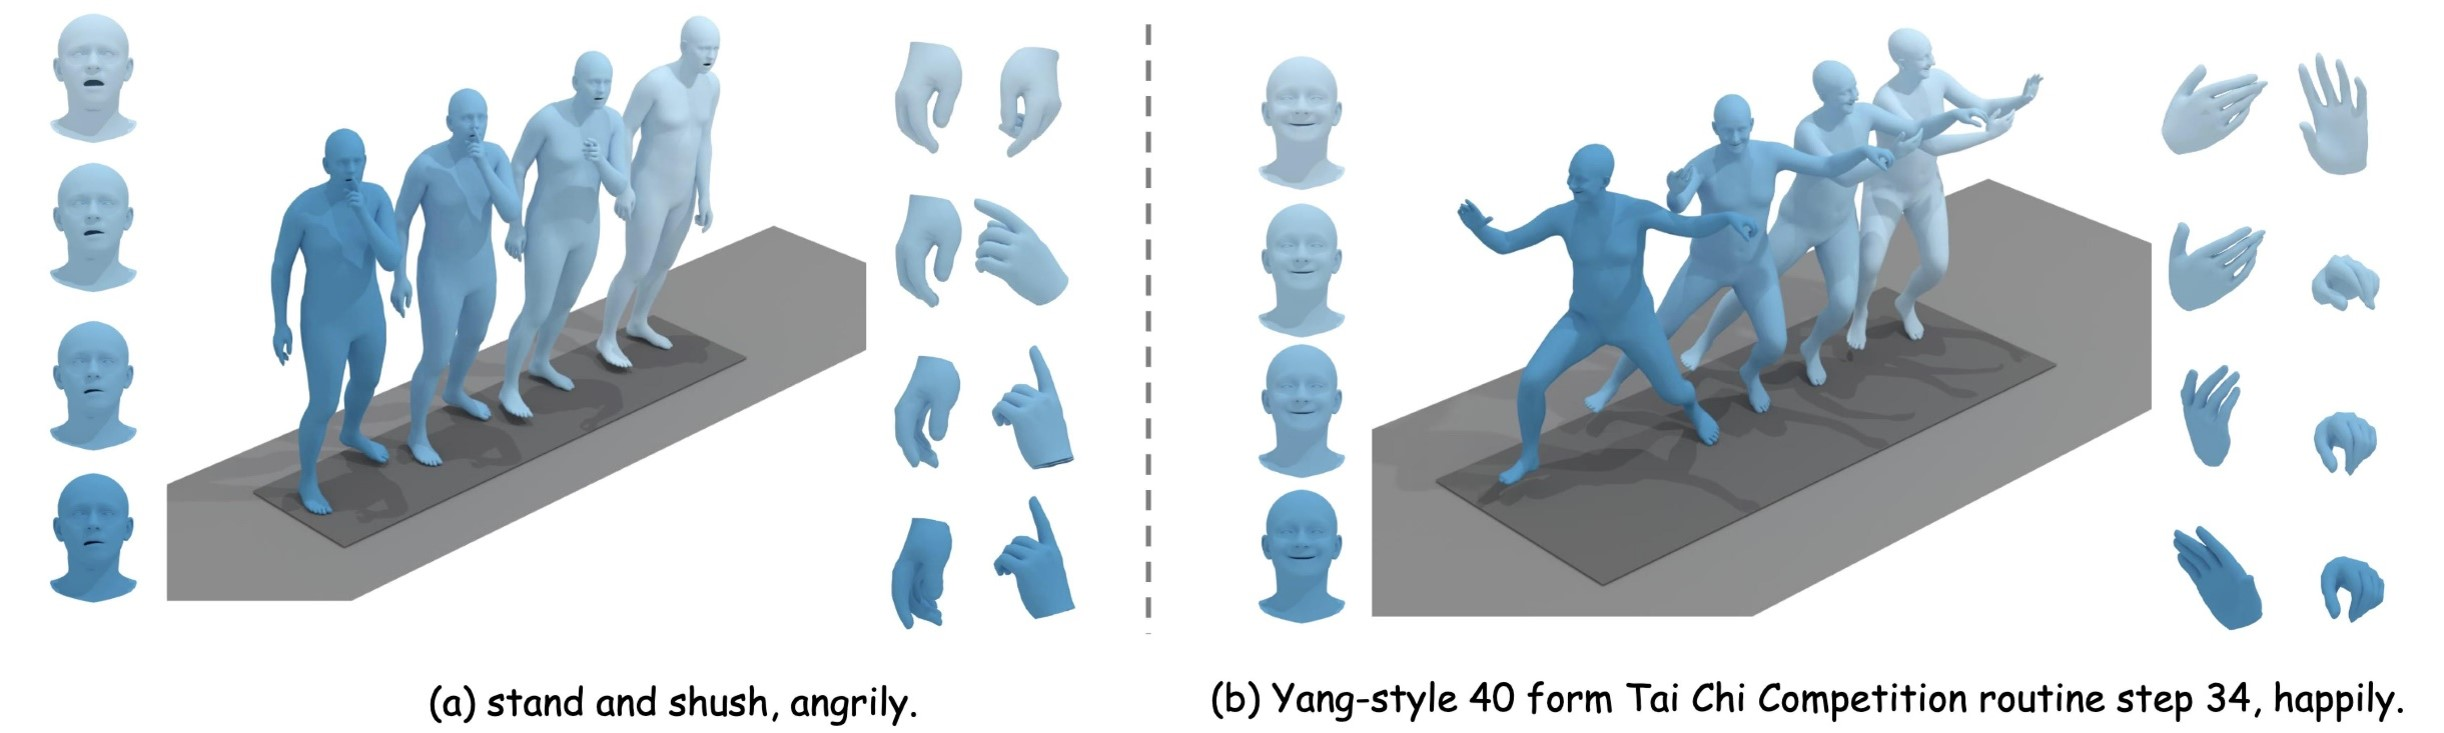
\includegraphics[width=\textwidth]{figs/mission.jpg}
    \caption{Human motions with different textual prompts\cite{lin2024motion}.}
    \label{fig:mission}
\end{figure}

% \begin{figure}[ht]
%     \centering
%     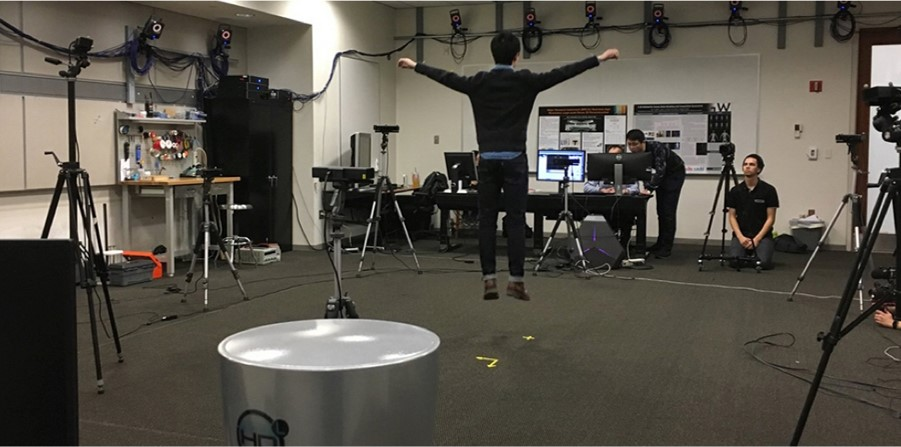
\includegraphics[width=\textwidth]{figs/mocap.jpg}
%     \caption{Illustration of the 3D motion capture process.}
%     \label{fig:mocap}
% \end{figure}

My 9-month work has been published for poster presentation at the ECCV 2024 Workshop: T. Sun et al., 'MCRE: Multimodal Conditional Representation and Editing for Text-Motion Generation,' ECCV Workshop on Foundation Models for 3D Humans, Sep. 2024.

\newpage 

\subsection{Goal}

The high-level goal for this doctoral research is to create a comprehensive system for generating realistic and animatable digital humans, enabling high-quality 3D avatars that are controllable through multimodal inputs, with applications across virtual reality, gaming, and social robotics. The project focuses on pushing the boundaries of model flexibility, control, and capability, contributing to the next generation of interactive digital human technologies.

\subsubsection{Goals for the First Year}
During the first year of my PhD, the research focused on laying a strong foundation for 3D human motion generation using multimodal approaches. A comprehensive literature review was conducted, exploring the state of the art in human motion generation, including models based on Variational Autoencoders (VAEs), tokenization-based approaches, and diffusion models. This review helped identify existing gaps and opportunities for advancing the field.

In addition, a novel framework for text-to-motion generation and editing was developed, supporting multiple tasks such as text-driven motion generation and motion completion. The core of this effort was the proposal and implementation of the Multimodal Conditional Representation and Editing (MCRE) framework. The MCRE framework integrates both text and motion data using foundation models, such as CLIP, to achieve precise multimodal control. To facilitate effective integration of multimodal conditions, a lightweight transformer module was also designed and implemented to align motion data to a shared representation space.

\subsubsection{Goals for the future}
The primary goal for the next year of this doctoral research is to continue advancing the development of multimodal approaches for 3D human motion generation, with a focus on enhancing flexibility, control, and generalization. The research will explore the integration of foundation models such as SVD \cite{blattmann2023stable} or Meta Movie Gen \cite{meta_movie_generation} to incorporate motion priors from 2D video data, aiming to enhance the model's text-to-motion synthesis capabilities. Leveraging these priors is expected to create more versatile models capable of handling various motion generation and editing tasks. This is one of the key focuses for the next nine months, with an expected completion by August 2025.

Another important goal is to expand the capabilities of motion transform to include stylized avatars, particularly focusing on driving avatars with complex appearances, such as loose clothing. By incorporating hybrid representations and leveraging geometric priors \cite{loper2023smpl}, this research aims to improve the ability to transfer skeletal motions to diverse avatar styles, thereby enhancing their animation quality and enabling them to handle intricate deformations effectively. This objective will also be a key focus over the next nine months, targeting completion by August 2025.

Addressing the challenge of generating long motion sequences is a key focus for the third phase of the doctoral program. Current models are typically constrained to short sequences, which limits their practical applications. The proposed research will develop methods to generate longer, coherent sequences, ensuring smooth transitions between segments, which is critical for applications like virtual avatars and gaming. This phase is scheduled to commence in late 2025 and will extend into 2026. During this time, the framework will be designed to integrate earlier findings and advancements from the first two years of research, consolidating the developed techniques to address the challenge of long sequence generation comprehensively. Completion of this framework is anticipated by mid-2026, depending on the outcomes of initial experiments and iterations.


\newpage 

\subsection{Contributions}
The key contributions of the work conducted over the past nine months are as follows:
\begin{itemize}
    \item Developed a framework for text-to-motion generation and editing that supports multiple tasks, including text-driven motion generation and motion completion.
    \item Designed and implemented a novel module for multimodal control, allowing for flexible manipulation of motion sequences using both text and motion inputs. This module demonstrated improved performance over baseline models in text-to-motion generation tasks, particularly in evaluations conducted on the HumanML3D dataset.
    \item Conducted experiments using motion capture datasets with caption, such as HumanML3D and Motion-X, demonstrating the system’s ability to handle complex text-driven motion tasks with high generalization performance.
\end{itemize}

\newpage 

\begin{figure}[h]
    \centering
    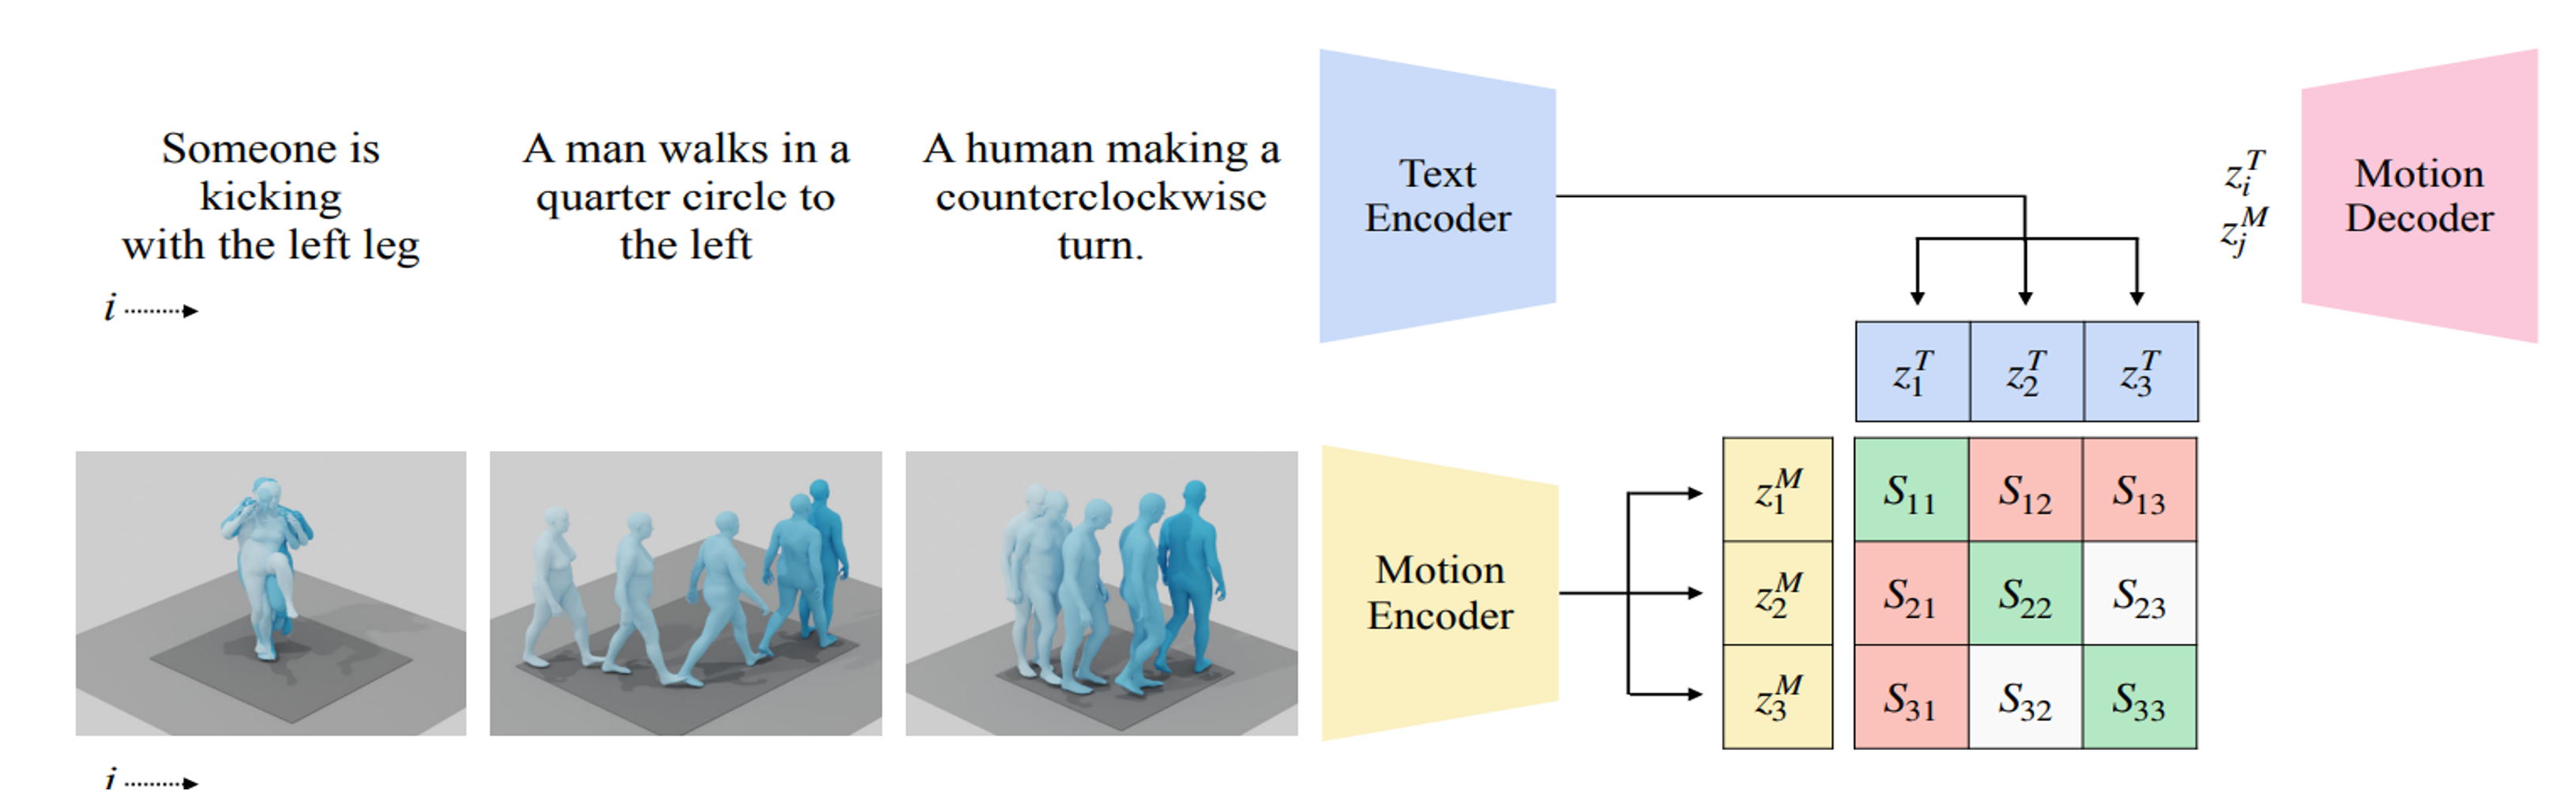
\includegraphics[width=\textwidth]{figs/TMR.png}
    \caption{TMR: Text-to-Motion Retrieval Using Contrastive 3D Human Motion Synthesis\cite{petrovich2023tmr}}
    \label{fig:TMR}
\end{figure}

\begin{figure}[h]
    \centering
    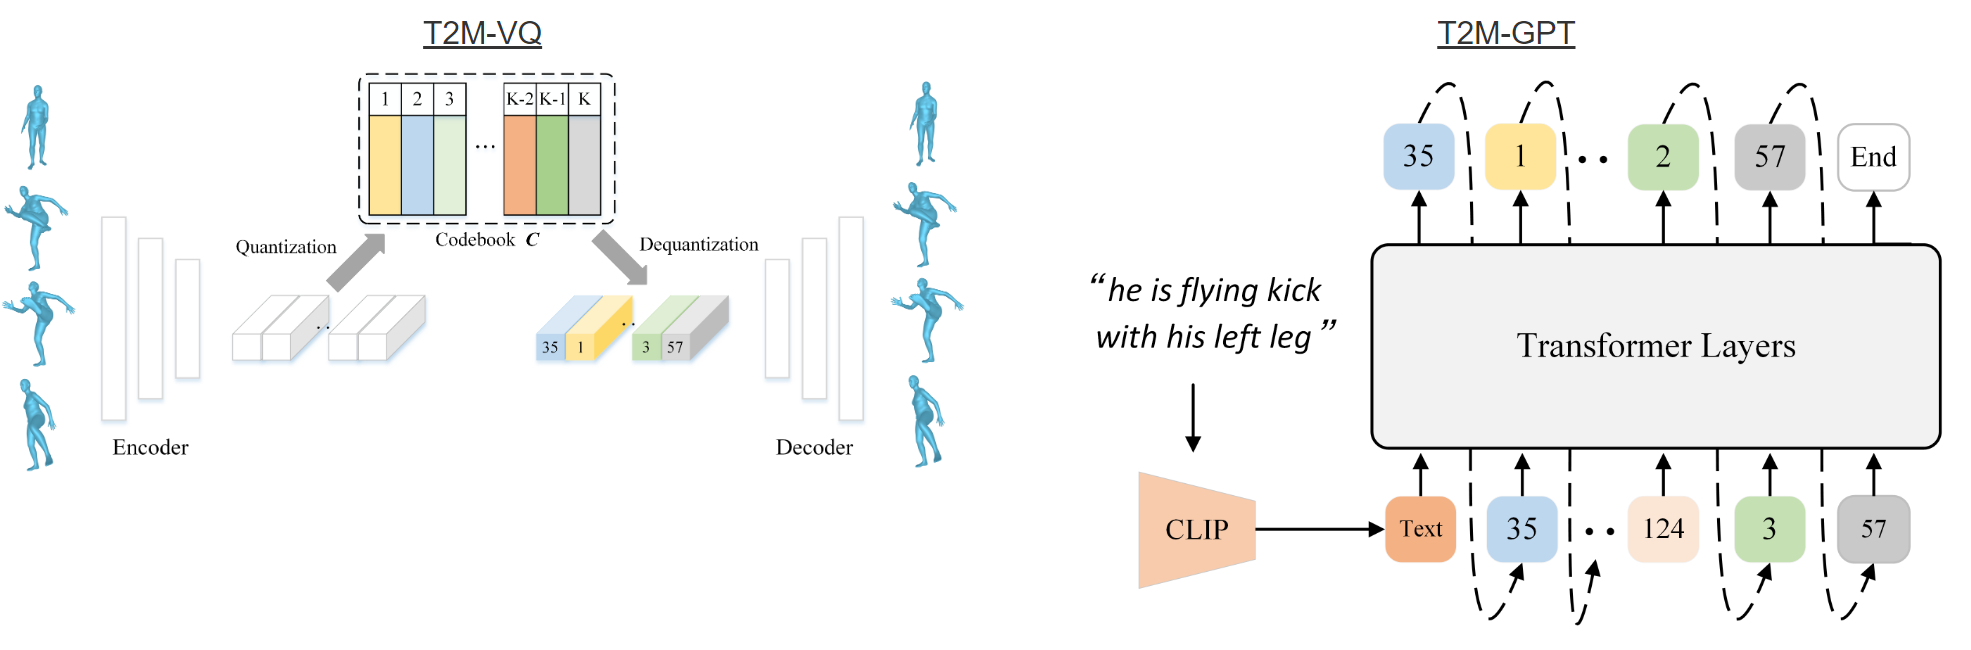
\includegraphics[width=\textwidth]{figs/T2M-GPT.png}
    \caption{T2M-GPT: Text-to-Motion Generation using Transformer-based Language Models\cite{zhang2023generating}.}
    \label{fig:T2M-GPT}
\end{figure}

\begin{figure}[h]
    \centering
    \includegraphics[width=\textwidth]{figs/MDM.png}
    \caption{MDM: Motion Diffusion Model for text-to-motion generation\cite{tevet2022human}.}
    \label{fig:MDM}
\end{figure}

\section{Related Work}

\subsection{Human Motion Generation}
Human motion generation has applications in virtual reality, animation, and robotics. Text is an intuitive interface for generating human motion, making text-to-motion generation an active research area.

As illustrated in Figure \ref{fig:TMR}, variational autoencoders (VAEs)\cite{kingma2013auto} are widely used for cross-modal generation, including human motion. VAEs encode input data into a latent space and decode it back, enabling diverse human motion generation. Notable examples include TEMOS\cite{petrovich2022temos} and TMR\cite{petrovich2023tmr}, which generate human motions from text or other motion inputs, offering an efficient alternative to diffusion-based models. Compared to diffusion models, VAEs are computationally ·efficient with faster inference, though they may lack fine-grained control.

As depicted in Figure \ref{fig:T2M-GPT}, tokenization-based methods convert motion sequences into discrete tokens, similar to natural language processing. These methods often use VQ-VAE, a VAE with a discrete latent space, to tokenize motion sequences. Models like MotionGPT\cite{jiang2024motiongpt} and T2M-GPT\cite{zhang2023generating} use transformers to process these tokens and generate motions based on text. While leveraging transformers enables high-quality outputs, the discrete space impacts motion smoothness, and autoregressive operations can accumulate errors, especially for long texts.

Diffusion-based methods have shown success in generating high-quality and diverse outputs, as shown in Figure \ref{fig:MDM}. Models such as MDM\cite{tevet2022human} and MotionDiffuse\cite{zhang2024motiondiffuse} apply diffusion models for text-to-motion generation, achieving promising results. MLD\cite{chen2023executing} further enhances performance by projecting motion data into a latent space before applying diffusion. However, these approaches generally focus on single-task generation and lack flexibility for multimodal inputs or complex control conditions.

\begin{figure}[ht]
    \centering
    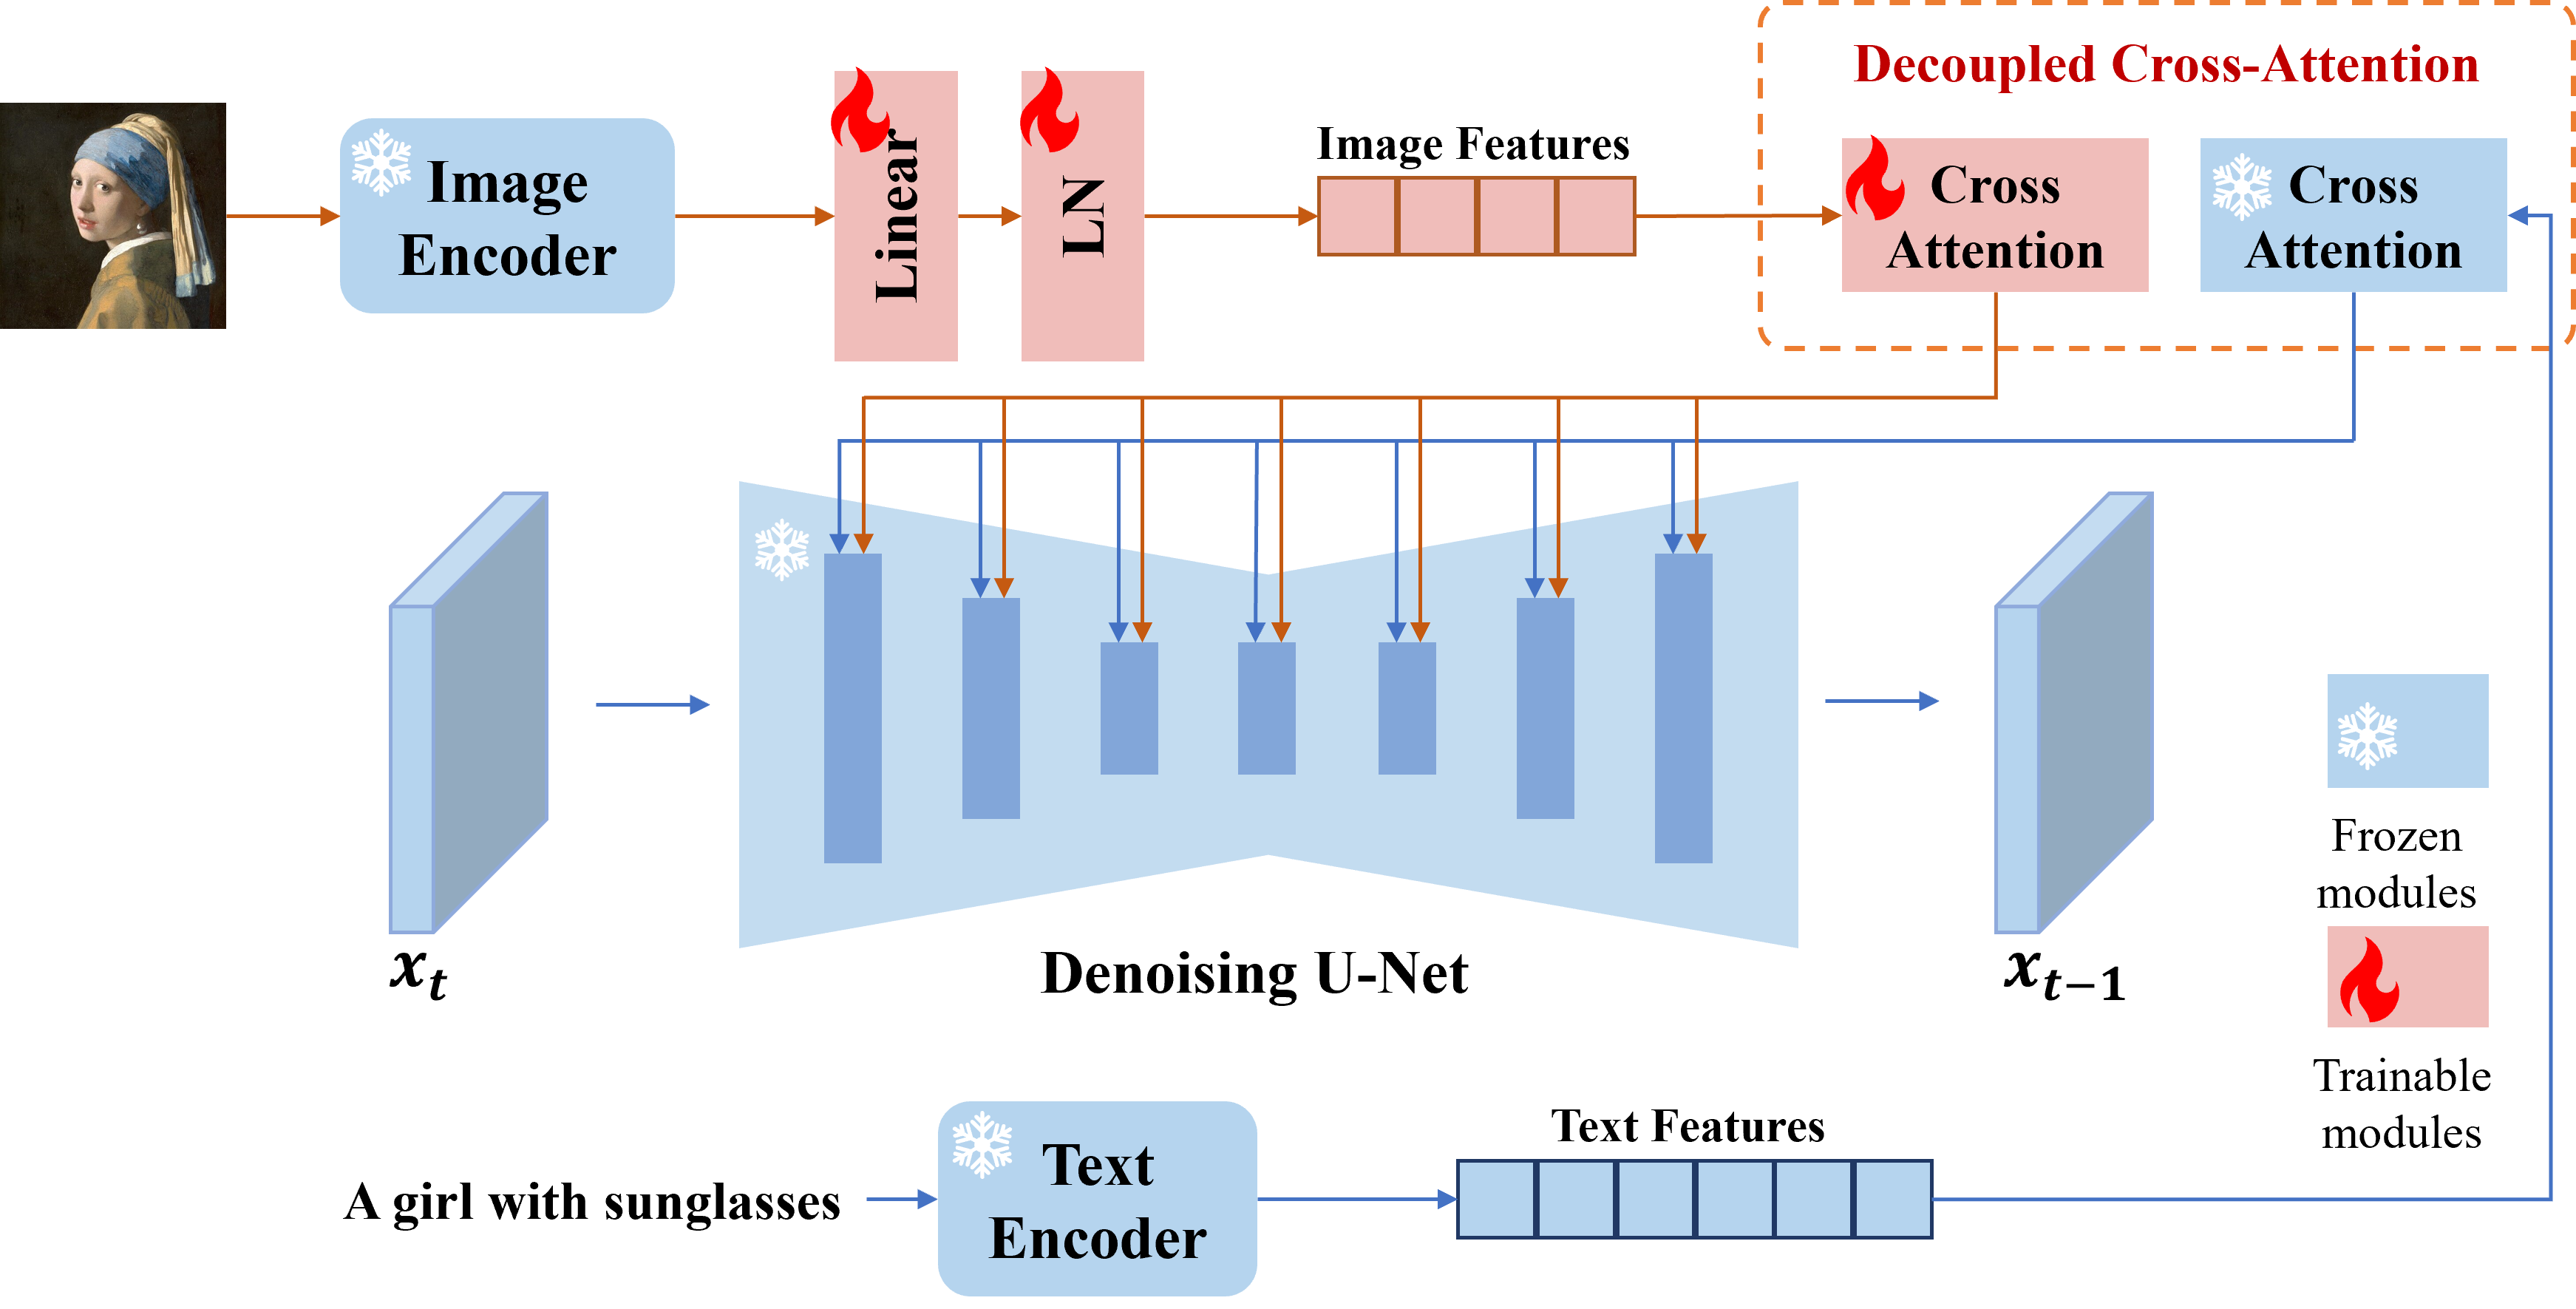
\includegraphics[width=\textwidth]{figs/ipadapter.png}
    \caption{IP-Adapter: Decoupled cross-attention mechanism for flexible prompt handling\cite{ye2023ip}.}
    \label{fig:ipadapter}
\end{figure}

\subsection{Adapter-based Approaches}
Recent research has explored the use of lightweight adapter modules to extend the capabilities of pre-trained generative models without requiring extensive retraining. These adapters provide flexibility by allowing additional control or functionality in the generation process.

As illustrated in Figure \ref{fig:ipadapter}, IP-Adapter \cite{ye2023ip} introduces a decoupled cross-attention mechanism that allows for image prompt handling while maintaining the text-to-image generation capabilities of the underlying model. Similarly, ControlNet \cite{zhang2023adding} enhances generation control by integrating additional input conditions, such as edge maps or keypoints, enabling greater manipulation of generated outputs.

\subsection{Multimodal Integration and Control}
In the field of text-to-image generation, adapter-based models such as T2I-Adapter \cite{mou2024t2i} incorporate both style and content features from reference images, merging them with text features to produce contextually appropriate outputs. This approach highlights the flexibility adapters offer by enabling seamless integration of multimodal inputs into the generation process.

Additionally, Prompt-to-Prompt \cite{hertz2022prompt} facilitates content manipulation by adjusting the embeddings of text prompts, allowing for style or content transfer between generated outputs without the need for extensive model retraining. This method further emphasizes the potential of adapters to enhance the control and flexibility of generative models.

These adapter-based methods demonstrate the potential for improving flexibility and performance in generative models. By enabling more fine-grained control and allowing for multimodal interactions, they provide a foundation for advancing text-to-motion generation systems. The integration of adapters into existing diffusion-based frameworks presents a promising direction for developing models capable of handling more complex control conditions and diverse tasks.

\newpage 

\section{Methodology}

This section will lay out the methods and techniques in implementations and experiments that have been done so far. This work has been accepted by ECCV 2024 Workshop on Foundation Models for 3D Humans.

As illustrated in Figure \ref{fig:whole_framework}, the model architecture used for 3D motion generation builds on the Multimodal Conditional Representation and Editing (MCRE) framework, which I propose to achieve precise multimodal control over the generation process. To enhance flexibility, I introduce the use of both text and existing motion data as control conditions. MCRE unifies text and motion data into a common representation space using the CLIP model, leveraging its strong semantic understanding and generalization capabilities. This approach facilitates effective integration of multimodal conditions, allowing for high-quality motion editing and generation.

For text conditions \( I_t^c \), I directly use the pre-trained CLIP text encoder to obtain condition representations in the CLIP space: \( c = CLIP_t(I_t^c) \). For motion conditions \( I_m^c \), I train an adapter \( W \) to align them with the CLIP space. This adapter employs a transformer encoder architecture. The adapter takes the action sequence and a learnable token as input, and the first token of the adapter output is taken as the final result: \( c = W(I_m^c) \). As illustrated in Figure \ref{fig:motion_adapter}, the lightweight transformer module aligns motion data to the CLIP representation space.

The training data for the adapter consists of pairs of text and motions. The training objective is to minimize the cosine distance between the CLIP embedding of the text and the adapter's output for the motion, defined as:
\begin{equation}
  L = 1 - \cos(CLIP_t(I_t^c), W(I_m^c))
\end{equation}

\begin{figure}[h]
    \centering
    \includegraphics[width=\textwidth]{figs/whole framework.png}
    \caption{Overview of the proposed MCRE framework for multimodal 3D motion generation.}
    \label{fig:whole_framework}
\end{figure}

\begin{figure}[h]
    \centering
    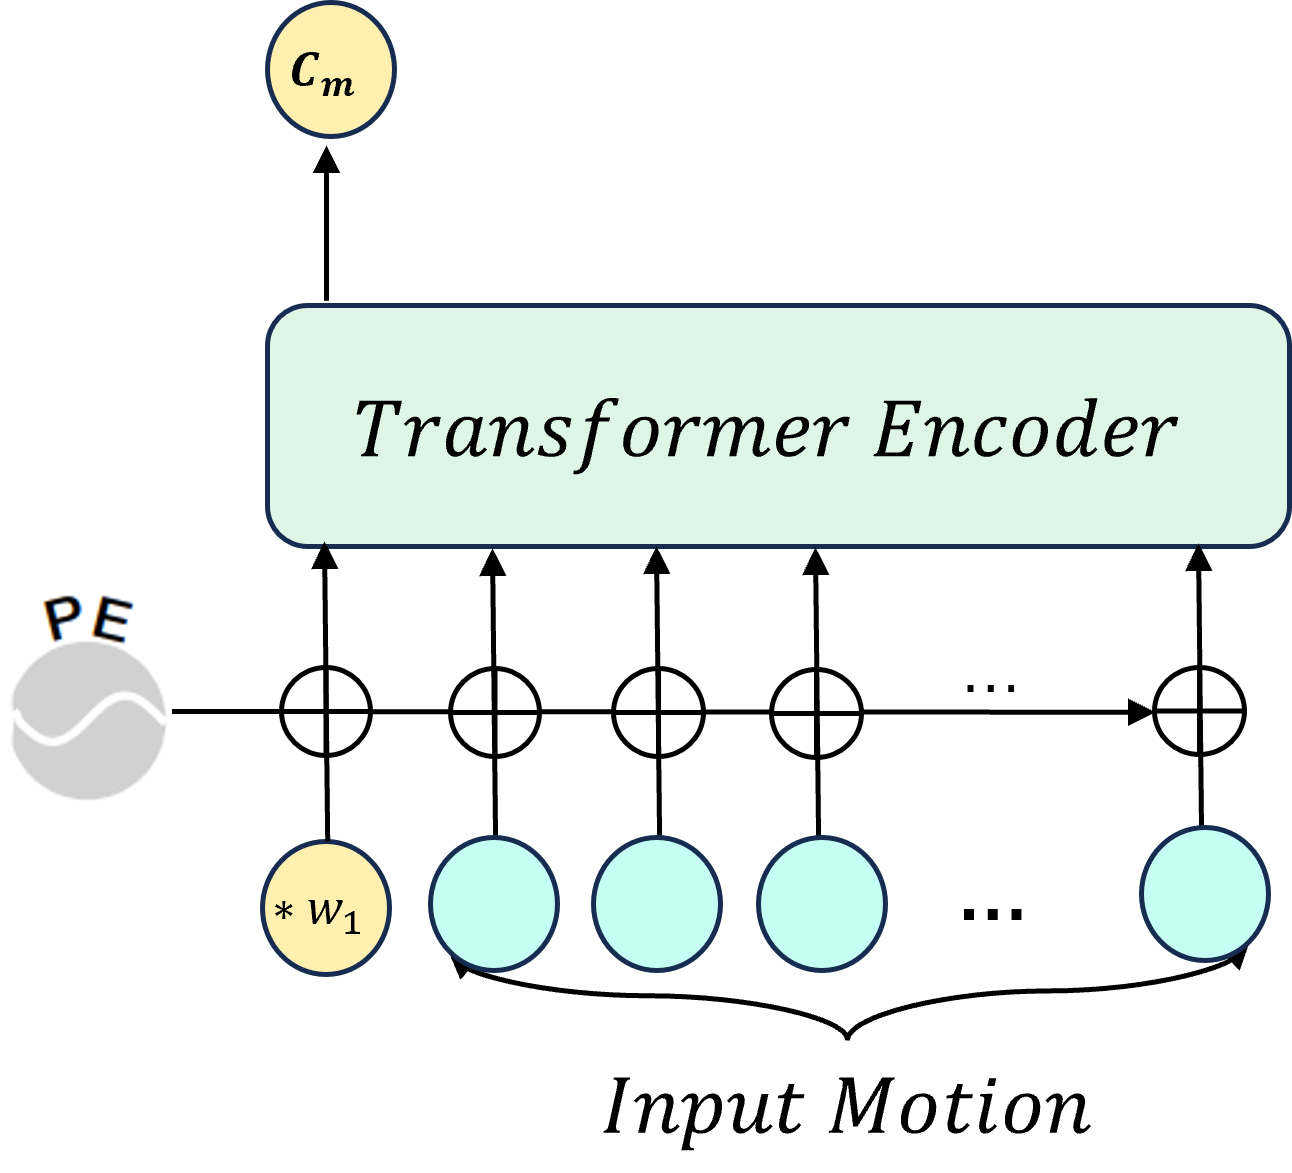
\includegraphics[width=0.45\textwidth]{figs/motion adapter.png}
    \caption{Lightweight transformer module for aligning motion data to the CLIP representation space.}
    \label{fig:motion_adapter}
\end{figure}

I use cosine loss to align the motion to their corresponding text representations in the CLIP space, ensuring that the adapter learns to map motion data effectively into the multi-modal representation space.


\subsection{Motion Editing via Multi-modal Conditional Editing}

The CLIP space exhibits highly disentangled characteristics, allowing us to perform various motion editing tasks through simple linear operations on the conditional CLIP representations. Specifically, to obtain the edited conditional representation \( c_{edit} \), I add the desired editing direction vector \( \Delta c_{edit} \) to the original motion representation:
\begin{equation} \label{eqa11}
c_{edit} = c + \Delta c_{edit}
\end{equation}
The edited conditional representation obtained in this way enables us to control the diffusion process to achieve the desired editing result. The editing direction is derived from the difference between the CLIP embeddings of the original and target conditions, which can be based on either text or motion.

Initially, I obtain the CLIP embeddings for text conditions using the pre-trained CLIP text encoder. For motion conditions, I train a transformer-based adapter to align motion data with the CLIP space. This involves minimizing the cosine distance between the text and motion embeddings during training. Once aligned, I can perform motion editing by calculating the difference between the CLIP embeddings of the target and original conditions, applying this difference to the original motion representation. This method leverages the semantic richness of the CLIP model, allowing for flexible and precise multimodal control over the generated motions.

\newpage 



\section{Experiments}
\subsection{Experimental Setup}
\textbf{Datasets.} I conducted experiments on two datasets: HumanML3D \cite{9880214} and Motion-X. I trained our model on the standard 3D human motion-language dataset, HumanML3D, which was derived from the HumanAct12 and AMASS datasets. Additionally, I processed a subset of Motion-X, consisting of 2.4k motions annotated with detailed textual descriptions, for the open-world generation experiment to evaluate the model's generalization.\\
\\
\textbf{Evaluation Metrics}. To evaluate the quality of rendered motions, I used the Frechet Inception Distance (FID) metric to measure the distribution distance between generated and original motions, considering both mean and variance. Additionally, Motion-Retrieval Precision (R-Precision) was used to assess the accuracy of generated motions in matching test prompts. Furthermore, I introduced the Motion Editing Consistency (MEC) metric to evaluate semantic similarity between edited motions and target text in the CLIP space. I also employed MM-Dist to measure the alignment between generated and original motion distributions. The Diversity metric \cite{9880214} ensures variety by assessing feature space variance. Finally, MModality evaluates the model's capability to generate motions matching various described categories, highlighting its versatility and robustness.\\
\\
\textbf{Comparison Methods.} I compared our functions with various baselines. For text-to-motion generation, I utilized MDM \cite{tevet2022human}, MotionDiffuse \cite{zhang2024motiondiffuse}, and MLD \cite{chen2023executing} to compare with our MCRE module combined with MLD.\\

\textbf{Experimental Details.} The MCRE module employs the pre-trained and frozen CLIP-ViT-B/32 model for the text encoder, while an eight-layer transformer network serves as the motion adapter. The dimensionality of the CLIP representation is \( c \in \mathbb{R}^{1 \times 512} \). Model training was conducted using the Adam optimizer \cite{lei2015adam}, with a learning rate of 0.0002 and a batch size of 128. Training of the MCRE module was performed on an RTX 4090 GPU, utilizing the HumanML3D dataset. The training of 100 epochs took approximately one hour to complete.

\begin{figure}[ht]
    \centering
    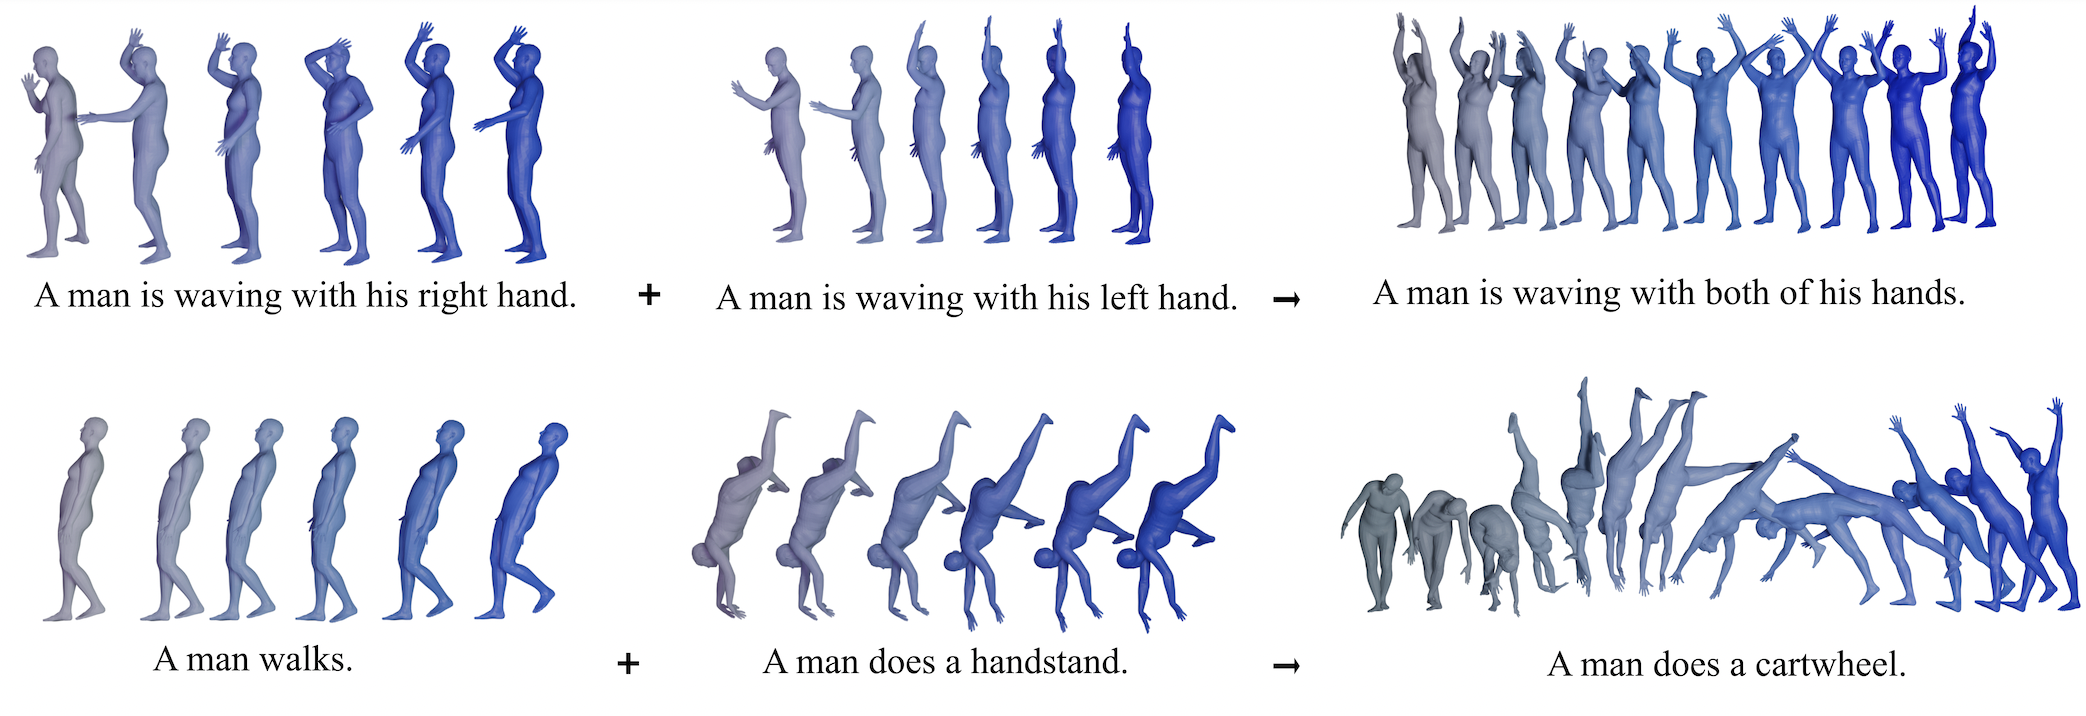
\includegraphics[scale=0.32]{figs/Linear_Combination.png}
    \caption{Linear Motion Combination.}
    \label{fig_linear_comb}
\end{figure}

\begin{figure}[ht]
    \centering
    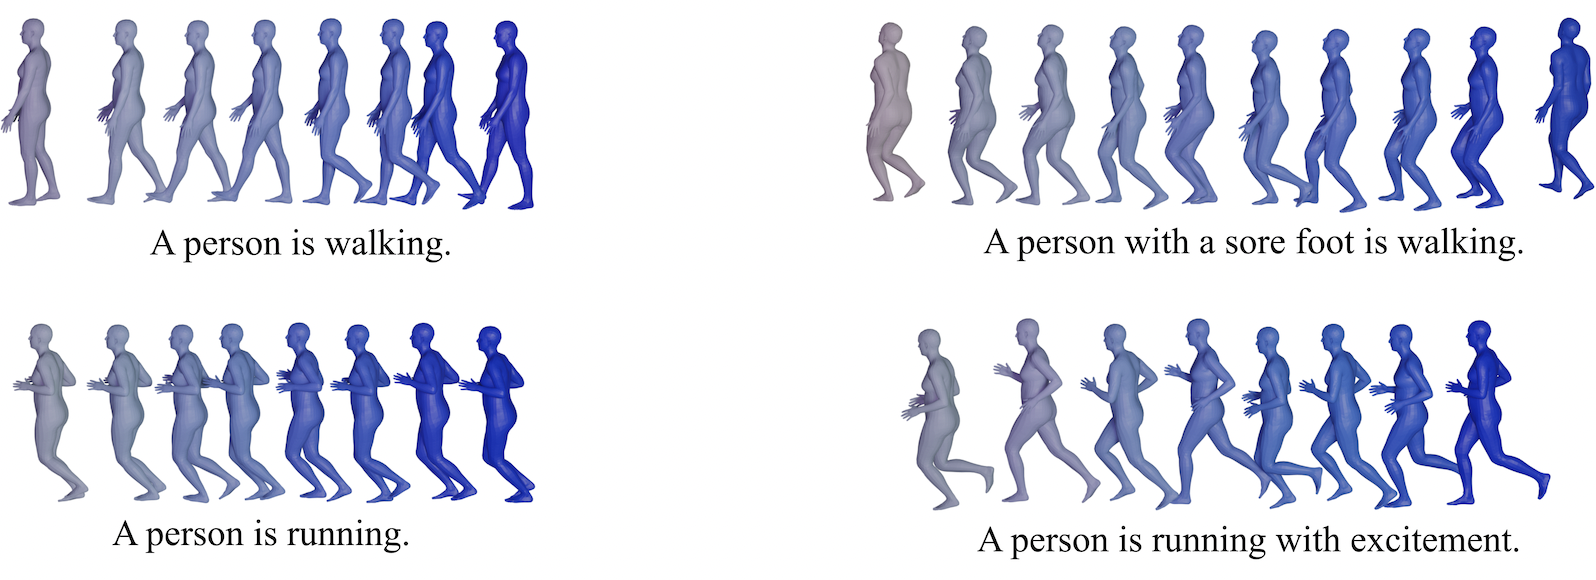
\includegraphics[scale=0.38]{figs/Montion_Edition.png}
    \caption{Motion Edition with additional conditions.}
    \label{fig_montion_edition}
\end{figure}


\subsection{Preliminary Results}
\subsubsection{Qualitative Evaluations}
With the assistance of the MCRE module, our model can synthesize complex motions from multiple simple text prompts. As illustrated in Figure \ref{fig_linear_comb}, the model processed the input descriptions ``A man is waving with his left hand'' and ``A man is waving with his right hand,'' generated a smooth motion through linear combinations and resulted in a depiction of a man waving with both hands. Additionally, given the prompts ``A man walks.'' and ``A man does a handstand.,'' the model successfully combined these actions to produce a coherent and realistic new motion, such as ``A man does a cartwheel.'' \\

Figure \ref{fig_montion_edition} demonstrates the motion editing capabilities of our model under various conditions. The top-left sequence shows a person walking normally. The top-right sequence depicts ``a person walking with a sore foot'', illustrating the model's ability to modify the motion to reflect physical discomfort. The bottom-left sequence presents a person running, while the bottom-right sequence shows a person running with excitement, highlighting the model's capacity to incorporate emotional states into the generated motions. This figure effectively showcases the versatility and precision of our motion editing system in adapting to both physical and emotional conditions.

\begin{table*}
  \caption{Quantitative results on the HumanML3D  test set}
  \label{tab1}
\begin{adjustbox}{width=1\textwidth}
\begin{tabular}{lccccccc}
\toprule
\multirow{2}{*}{Method} & \multicolumn{3}{c}{R-Precision$\uparrow$}                                                & \multicolumn{1}{l}{\multirow{2}{*}{FID$\downarrow$}} & \multicolumn{1}{l}{\multirow{2}{*}{MM-Dist$\downarrow$}} & \multicolumn{1}{l}{\multirow{2}{*}{Diversity$\rightarrow$}} & \multicolumn{1}{l}{\multirow{2}{*}{ MModality$\uparrow$}} \\ 
                        & \multicolumn{1}{l}{Top1} & \multicolumn{1}{l}{Top2} & \multicolumn{1}{l}{Top3} & \multicolumn{1}{l}{}                     & \multicolumn{1}{l}{}                         & \multicolumn{1}{l}{}                           & \multicolumn{1}{l}{}                           \\ \midrule
"HumanML3D Test set" \\
\midrule
Real & $0.511^{\pm.003}$ & $0.703^{\pm.003}$ & $0.797^{\pm.002}$ & $0.002^{\pm.000}$ & $2.974^{\pm.008}$  & $9.503^{\pm.065}$ & - \\ \hdashline
\rule{0pt}{10pt}MDM \cite{tevet2022human}  & $0.320^{\pm.005}$  & $0.498^{\pm.004}$ & $0.611^{\pm.007}$  & $0.544^{\pm.044}$  & $5.566^{\pm.027}$  & $\underline{9.559}^{\pm.086}$  & $\textbf{2.799}^{\pm.072}$                                          \\
MotionDiffuse \cite{zhang2024motiondiffuse}           & $\underline{0.491}^{\pm.001}$                    & $\underline{0.681}^{\pm.001}$                    & $\textbf{0.782}^{\pm.001}$                    & $0.630^{\pm.001}$                                    & $\underline{3.113}^{\pm.001}$                                        & $9.410^{\pm.049}$                                          & $1.553^{\pm.042}$                                          \\
MLD \cite{chen2023executing}                     & $0.481^{\pm.003}$                    & $0.673^{\pm.003}$                    & $0.772^{\pm.002}$                    & $\underline{0.473}^{\pm.013}$                                    & $3.196^{\pm.010}$                                        & $9.724^{\pm.082}$                                          & $2.413^{\pm.079}$                                          \\
Ours                    & $\textbf{0.499}^{\pm.003}$                  & $\textbf{0.683}^{\pm.003}$                   & $\underline{0.780}^{\pm.002}$                    & $\textbf{0.339}^{\pm.009}$                                    & $\textbf{3.087}^{\pm.008}$                                        & $\textbf{9.527}^{\pm.053}$                                          & $\underline{2.500}^{\pm.083}$                                          \\ 
\midrule

\end{tabular}
\end{adjustbox}
\end{table*}


\subsubsection{Quantitative Evaluations}
I evaluated the performance with the dataset using the evaluation metrics and comparison methods introduced in Section 4.1. For text-motion generation task, as shown in Table \ref{tab1}, achieved superior results in R-Precision, FID, and MM-Dist, and also shows commendable diversity.

For motion editing evaluation, MEC involves generating a fused text description \( \text{T}_{\text{target}} \) for each pair of text-motion pairs using ChatGPT \cite{openai2024chatgpt}.

\begin{equation}
\text{T}_{\text{target}} = \text{ChatGPT}(I_{t1}^{c1}, I_{t2}^{c2})
\end{equation}

Subsequently, \( \text{M}_{\text{edit}} \) is generated by these two pairs of conditions. Finally, \( \text{T}_{\text{target}} \) and \( \text{M}_{\text{edit}} \) are input into MCRE, and the Euclidean distance between their embeddings is calculated as follows:

\begin{equation}
\text{MEC} = \text{Dist}\left(C_{\text{CLIP}}\left(\text{T}_{\text{target}}\right), W\left(\text{M}_{\text{edit}}\right)\right)
\end{equation}

Specifically, MEC leverages the alignment of motions and texts in the CLIP embedding space. During training, I aligned the motion data with the pre-trained textual embeddings in CLIP, ensuring that actions with similar semantics as described by text produce similar embeddings. Thus, by comparing the embeddings of the newly generated text and motion, I could quantify how well the edited motion matches the target description. A smaller Euclidean distance indicates higher semantic similarity, demonstrating the model's ability to produce motions that align closely with complex text prompts. After standardizing the data, our MEC evaluation results show an average distance of \(0.41^{\pm.028}\), indicating a high level of semantic consistency.

The newly designed MEC metric shows that our edited motions align well with the target descriptions in the CLIP space.


\newpage

\section{Discussion}
\subsection{Challenges and Observations}
One of the major challenges faced in this research is achieving a balance between model flexibility and output quality. While diffusion-based methods offer high-quality, diverse outputs, they are often limited by their focus on single-task generation, which restricts their adaptability for more complex, multimodal tasks. Addressing this issue requires innovative techniques to extend diffusion models beyond single-task settings and enable them to handle multimodal conditions seamlessly.

Another challenge is the inherent difference in the representation, dimensionality, and structure of text and motion data. Text data is sequential and often abstract, whereas motion data is high-dimensional and spatially continuous. This disparity poses difficulties in aligning the semantics of text with corresponding motion representations, leading to mismatches and inconsistencies during generation. Our proposed multimodal framework attempts to address this by leveraging foundation models for better generalization and alignment.

\subsection{Comparison with Existing Works}
Compared to existing methods, our approach aims to push the boundaries of flexibility in text-to-motion generation. Unlike VAE-based methods, which often lack control, our diffusion-based approach provides more fine-grained control over generated sequences. Additionally, while tokenization-based methods suffer from issues related to smoothness and error accumulation, our method operates in continuous space, allowing for smoother and more realistic outputs.

Our approach also differs from traditional diffusion-based models by extending beyond single-task generation. By integrating adapters mechanism, our framework can handle tasks like motion editing, completion, and multimodal controlled generation. This flexibility sets our work apart from current other methods, which primarily focus on generating motion sequences from text without enabling detailed editing or handling other modalities.

\newpage

\begin{figure}[ht]
    \centering
    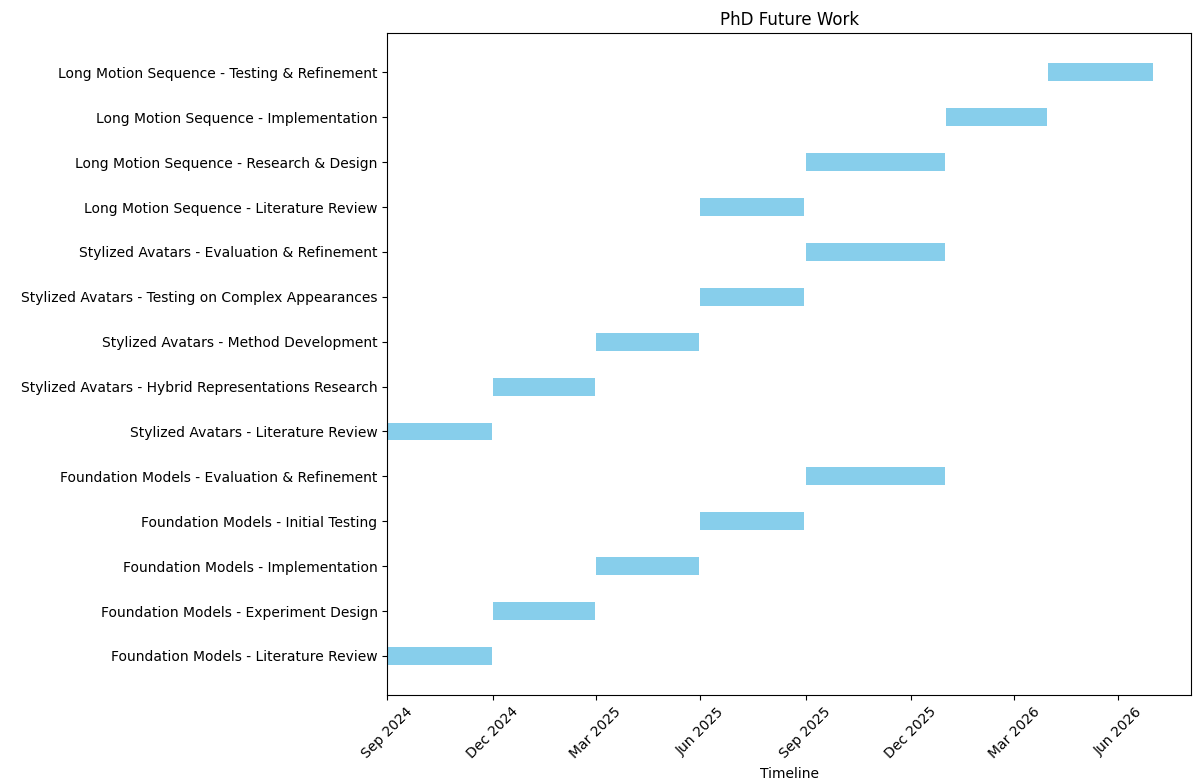
\includegraphics[width=\textwidth]{figs/Gantt.png}
    \caption{PhD Future Work Timeline.}
    \label{fig:gantt}
\end{figure}

\section{Future Work}

As shown in Figure \ref{fig:gantt}, the Gantt chart illustrates the detailed timeline for future work in the PhD project, including specific tasks such as the implementation of foundation models for motion synthesis, motion transform for stylized avatars, and long motion sequence generation.

\subsection{Foundation Models for Motion Synthesis}
Training models with limited motion data remains a bottleneck. Unlike text or image datasets, motion datasets are expensive to acquire and annotate, limiting the diversity of training data available. This scarcity can hinder the model’s ability to generalize to unseen motion styles or complex interactions. Data augmentation techniques, synthetic data generation, and transfer learning approaches are some of the strategies I am exploring to mitigate this challenge.

The first direction involves further exploring the impact of foundation models in enhancing motion synthesis tasks. Compared to 3D motion data, 2D images and videos related to human motion are more abundant and easier to acquire. Therefore, in the next phase of the research, I plan to design experiments that leverage video-based models, such as SVD \cite{blattmann2023stable} or Meta's newly open-sourced Meta Movie Gen \cite{meta_movie_generation} framework, to utilize motion priors from videos. This would help in enhancing the text-to-motion synthesis capabilities of our model. Additionally, I also aim to investigate tasks such as controlling motion generation and editing using video inputs.

In the next three months, I will conduct a comprehensive literature review on foundation models for 2D to 3D motion synthesis and begin designing experiments that incorporate video-based priors into the current framework. By the 18-month confirmation milestone, which will be in mid-2025, I aim to complete the initial implementation of models leveraging foundation models for text-to-motion synthesis and begin conducting experiments to assess their effectiveness.

\subsection{Motion Transform for Stylized Avatars}
In addition to motion synthesis, I plan to explore the use of motion transform techniques to animate stylized avatar models using skeletal motion \cite{li2024animatable, shao2024splattingavatar, svitov2024haha}. Current research in this area is relatively scarce, and there are still challenges when it comes to transferring motion captured from one setup to drive stylized avatars, particularly those with complex appearances such as loose clothing. This limitation often stems from the absence of comprehensive geometric priors. Novel 3D representations, like NeRF \cite{mildenhall2021nerf} and 3dgs \cite{kerbl20233d}, have shown promise in animatable digital human generation but struggle with handling these types of avatars. A potential solution involves hybrid representations that incorporate SMPL \cite{loper2023smpl} model geometric priors, although the SMPL model itself primarily focuses on the body trunk, which limits its effectiveness for other aspects of the avatar's appearance. Therefore, I plan to design a method that is better able to handle complex deformations in avatars during motion.

In the next three months, I will focus on the use of hybrid representations and geometric priors to better understand their limitations. By the 18-month confirmation, I aim to develop and test an initial method for motion transformation on stylized avatars, especially targeting intricate appearances like loose clothing.

\subsection{Long Motion Sequence Generation}
Generating long motion sequences represents an important but challenging aspect of this research. Current models are constrained to short sequences, typically limited to about 12 seconds, which restricts practical applications. Breaking up sequences into multiple segments introduces the challenge of ensuring seamless transitions between segments. The development of a framework capable of generating longer and more coherent motion sequences will be crucial, particularly for applications in virtual avatars and gaming.

Given the importance of addressing these challenges, I plan to focus on the framework for long sequence generation between the 18-month and 30-month periods of my PhD, starting from mid-2025. During this phase, I will explore the use of traditional motion prediction techniques to assist in achieving coherence across longer sequences. The integration of findings from earlier research—such as motion priors from foundation models and techniques for handling stylized avatars—will also be part of this framework, making it a comprehensive solution for long-term sequence generation. The anticipated completion for this framework is by mid-2026, allowing time for iterative testing and refinement.


\bibliographystyle{plain}
\bibliography{references}

\end{document}
